\documentclass[12pt, a4paper, simple]{eskdtext}

\usepackage{env}
\usepackage{_sty/gpi_lstlisting}
\usepackage{hyperref}

% Код
\def \gpiDocTypeNum {81}
\def \gpiDocVer {00}
\def \gpiCode {\gpiLetterI\gpieLetterII\gpiLetterIII.\gpiStudentGroupName\gpiStudentGroupNum.\gpiStudentCard.0\gpiDocNum~\gpiDocTypeNum~\gpiDocVer}

\def \gpiDocTopic {ОТЧЁТ ЛАБОРАТОРНОЙ РАБОТЫ №\gpiDocNum}

% Графа 1 (наименование изделия/документа)
\ESKDcolumnI {\ESKDfontII \gpiTopic \\ \gpiDocTopic}

% Графа 2 (обозначение документа)
\ESKDsignature {\gpiCode}

% Графа 4 (литералы)
\ESKDcolumnIVfI {\gpiLetterI}
\ESKDcolumnIVfII {\gpieLetterII}
\ESKDcolumnIVfIII {\gpiLetterIII}

% Графа 9 (наименование или различительный индекс предприятия) задает команда
\ESKDcolumnIX {\gpiDepartment}

% Графа 11 (фамилии лиц, подписывающих документ) задают команды
\ESKDcolumnXIfI {\gpiStudentSurname}
\ESKDcolumnXIfII {\gpiTeacherSurname}
\ESKDcolumnXIfV {\gpiTeacherSurname}

\begin{document}
    \begin{ESKDtitlePage}
    \begin{center}
        \gpiMinEdu \\
        \gpiEdu \\
        \gpiKaf \\
    \end{center}

    \vfill

    \begin{center}
        \gpiTopic
    \end{center}

    \vfill

    \begin{center}
        \textbf{\gpiDocTopic} \\
        ПО ДИСЦИПЛИНЕ \gpiDiscipline \\
    \end{center}

    \vfill

    \begin{flushright}
        \begin{minipage}[t]{7cm}
            Выполнил:\\
            \PageTitleStudentInfo
            \PageTitleDateField
            \hspace{0pt}

            Проверил:\\
            \PageTitleTeacherInfo
            \PageTitleDateField
        \end{minipage}
    \end{flushright}

    \vfill

    \begin{center}
        \PageTitleCity~\ESKDtheYear
    \end{center}
\end{ESKDtitlePage}

    \paragraph{Задание 1 Вариант 1} \hspace{0pt}

Применить паттерн абстрактная фабрика при построении схемы из простых графических объектов.
Продукты фабрики: прямоугольник, линия, овал, текст.

\begin{figure}[!htb]
    \centering
    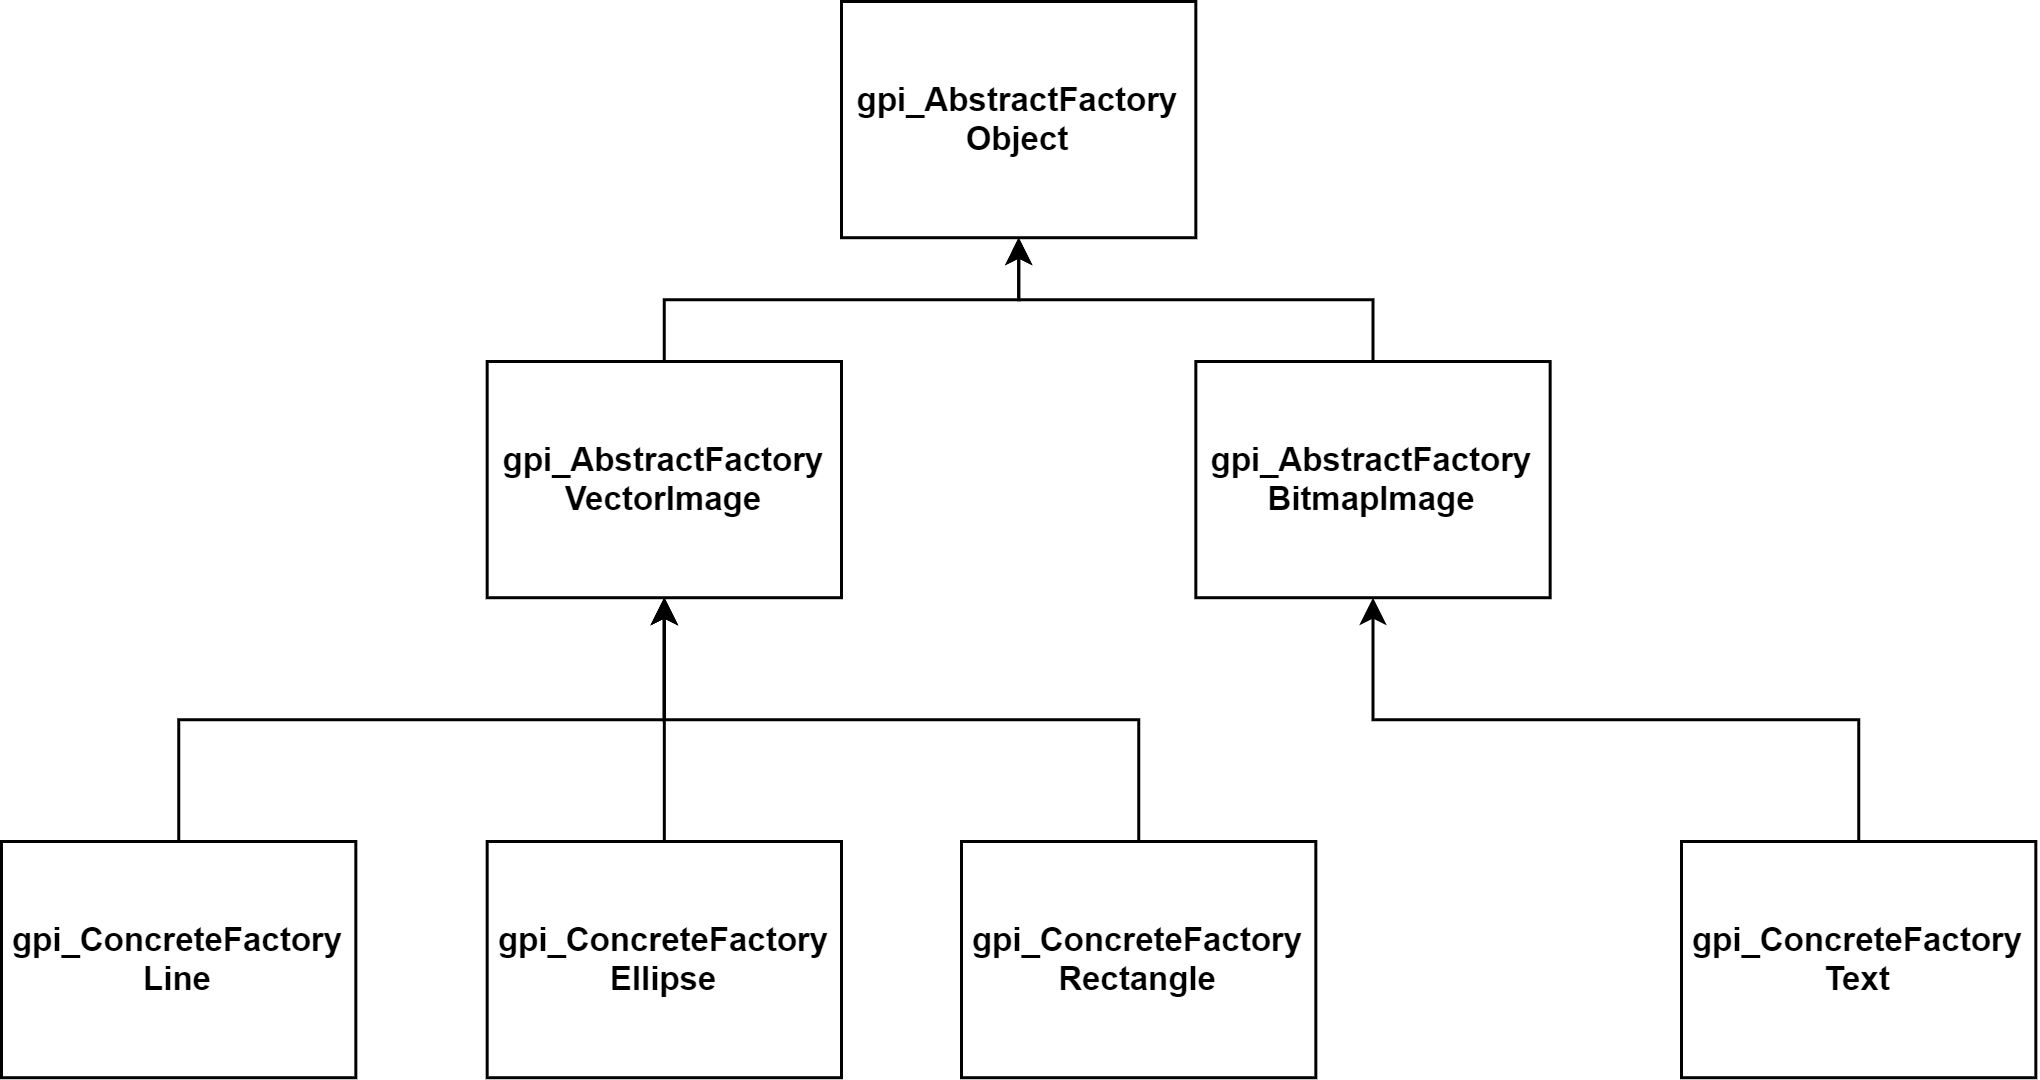
\includegraphics[width=16cm]
        {_assets/gpi_ootpisp5_lab8_task_1_1.png}
    \caption{Диаграмма наследования классов}
\end{figure}

\lstinputlisting[language=csh, name=Program.cs,]
{../gpi_ootpisp5_lab8_task_1_1/gpi_ootpisp5_lab8_task_1_1/Program.cs}

\lstinputlisting[language=csh, name=gpi_AbstractFactoryObject.cs,]
{../gpi_ootpisp5_lab8_task_1_1/gpi_ootpisp5_lab8_task_1_1/gpi_AbstractFactoryObject.cs}

\lstinputlisting[language=csh, name=gpi_AbstractFactoryBitmapImage.cs,]
{../gpi_ootpisp5_lab8_task_1_1/gpi_ootpisp5_lab8_task_1_1/gpi_AbstractFactoryBitmapImage.cs}

\lstinputlisting[language=csh, name=gpi_AbstractFactoryVectorImage.cs,]
{../gpi_ootpisp5_lab8_task_1_1/gpi_ootpisp5_lab8_task_1_1/gpi_AbstractFactoryVectorImage.cs}

\lstinputlisting[language=csh, name=gpi_ConcreteFactoryText.cs,]
{../gpi_ootpisp5_lab8_task_1_1/gpi_ootpisp5_lab8_task_1_1/gpi_ConcreteFactoryText.cs}

\lstinputlisting[language=csh, name=gpi_ConcreteFactoryLine.cs,]
{../gpi_ootpisp5_lab8_task_1_1/gpi_ootpisp5_lab8_task_1_1/gpi_ConcreteFactoryLine.cs}

\lstinputlisting[language=csh, name=gpi_ConcreteFactoryRectangle.cs,]
{../gpi_ootpisp5_lab8_task_1_1/gpi_ootpisp5_lab8_task_1_1/gpi_ConcreteFactoryRectangle.cs}

\lstinputlisting[language=csh, name=gpi_ConcreteFactoryEllipse.cs,]
{../gpi_ootpisp5_lab8_task_1_1/gpi_ootpisp5_lab8_task_1_1/gpi_ConcreteFactoryEllipse.cs}

\lstinputlisting[name=Console out,]
{_assets/gpi_ootpisp5_lab8_task_1_1.exe.txt}

\end{document}
